%%%%%%%%%%%%%%%%%%%%%%%%%%%%%%%%%%%%%%%%%
% Beamer Presentation
% LaTeX Template
% Version 1.0 (10/11/12)
%
% This template has been downloaded from:
% http://www.LaTeXTemplates.com
%
% License:
% CC BY-NC-SA 3.0 (http://creativecommons.org/licenses/by-nc-sa/3.0/)
%
%%%%%%%%%%%%%%%%%%%%%%%%%%%%%%%%%%%%%%%%%

%----------------------------------------------------------------------------------------
%	PACKAGES AND THEMES
%----------------------------------------------------------------------------------------

\documentclass{beamer}

\mode<presentation> {

% The Beamer class comes with a number of default slide themes
% which change the colors and layouts of slides. Below this is a list
% of all the themes, uncomment each in turn to see what they look like.


%\usetheme{Luebeck}
\usetheme{Madrid}
%\usetheme{Malmoe}
%\usetheme{Marburg}
}

% As well as themes, the Beamer class has a number of color themes
% for any slide theme. Uncomment each of these in turn to see how it
% changes the colors of your current slide theme.

%

%\setbeamertemplate{footline} % To remove the footer line in all slides uncomment this line
%\setbeamertemplate{footline}[page number] % To replace the footer line in all slides with a simple slide count uncomment this line

%\setbeamertemplate{navigation symbols}{} % To remove the navigation symbols from the bottom of all slides uncomment this line
\usepackage{xspace}
\usepackage{multicol}
\usepackage{amsmath,mathrsfs,amscd}
\usepackage{subfig}

\usepackage{slashed}
\usepackage{graphicx} % Allows including images
\usepackage{booktabs} % Allows the use of \toprule, \midrule and \bottomrule in tables
\usepackage[compat=1.1.0]{tikz-feynman}
\newcommand\Tstrut{\rule{0pt}{3.0ex}}         % = `top' strut
\newcommand\Bstrut{\rule[-1.5ex]{0pt}{0pt}}   % = `bottom' strut
\newcommand{\ftapprox}{FT$_{\mathrm{approx}}$\xspace}
\newcommand{\nnloBP}{NNLO$_{\mathrm{B-proj}}$\xspace}
\newcommand{\nnloNI}{NNLO$_{\mathrm{NLO-i}}$\xspace}
\newcommand{\nnloFT}{NNLO$_{\mathrm{FTapprox}}$\xspace}
\newcommand{\nloFT}{NLO$_{\mathrm{FTapprox}}$\xspace}
\newcommand{\sqrtS}{\ensuremath{\sqrt{s}}}
\def\E#1{\times 10^{#1}}

%----------------------------------------------------------------------------------------
%	TITLE PAGE
%----------------------------------------------------------------------------------------

\title[gammaH]{First Glance at $\gamma H$ Samples via JHU Generator} % The short title appears at the bottom of every slide, the full title is only on the title page

\author{Ren-Qi Pan} % Your name
\institute[ZJU] % Your institution as it will appear on the bottom of every slide, may be shorthand to save space
{
Zhejiang University\\ % Your institution for the title page
\medskip
%\textit{renqipan@zju.edu.cn} % Your email address
}
\date{\today} % Date, can be changed to a custom date
\pagenumbering{arabic}

\begin{document}

\begin{frame}
\titlepage % Print the title page as the first slide
\end{frame}

\begin{frame}
\begin{center}
\frametitle{Set up Parameters}
In SM: $a_{2}^{Z\gamma}=-0.007$, $a_{2}^{\gamma \gamma}=0.004$\\
Cite: Phys.Rev.D92(2015)012004\\
~\\
Scalar, $J^{P}=0^{+}$: $a_{2}^{Z\gamma}=-0.007$, $a_{2}^{\gamma \gamma}=0.004$\\
Pseudoscalar, $J^{P}=0^{-}$: $a_{3}^{Z\gamma}=-0.007$,  $a_{3}^{\gamma \gamma}=0.004$\\
\end{center}
\end{frame}

\begin{frame}
\frametitle{Cross section}
\begin{center}
Use JHU generator to generate weighted samples
$\sigma(\gamma^{*}\rightarrow\gamma H,J^{P}=0^{+})=2.8fb$\\
$\sigma(\gamma^{*}\rightarrow\gamma H,J^{P}=0^{-})=2.8fb$\\
~\\
$\sigma(Z^{*}\rightarrow\gamma H,J^{P}=0^{+})=14.6fb$\\
$\sigma(Z^{*}\rightarrow\gamma H,J^{P}=0^{-})=14.7fb$\\
~\\
Comparison: $\sigma(ZH)=0.88pb$, $\sigma(tth)=0.50pb$\\
Note: Data taken from PDG-2017


\end{center}
\end{frame}

\begin{frame}
\frametitle{Kinematics of Higgs}
\begin{figure}[H]
\setcounter{subfigure}{0}
\centering
\subfloat[Distribution of Higgs $\eta$ ]{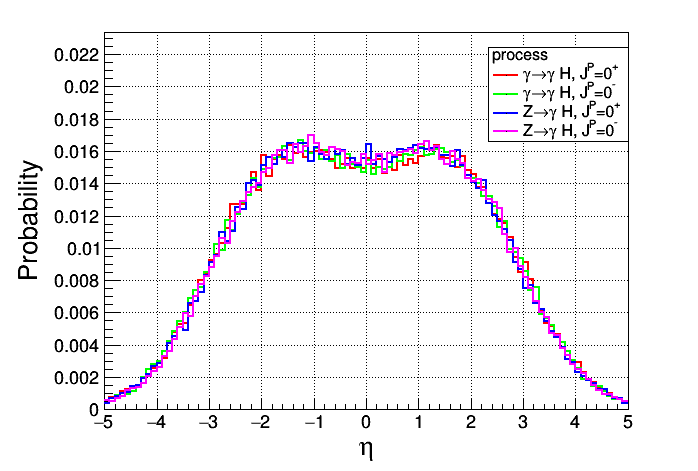
\includegraphics[width=0.45\textwidth]{./figures/h_eta}} 
\subfloat[Distribution of Higgs $p_T$ ]{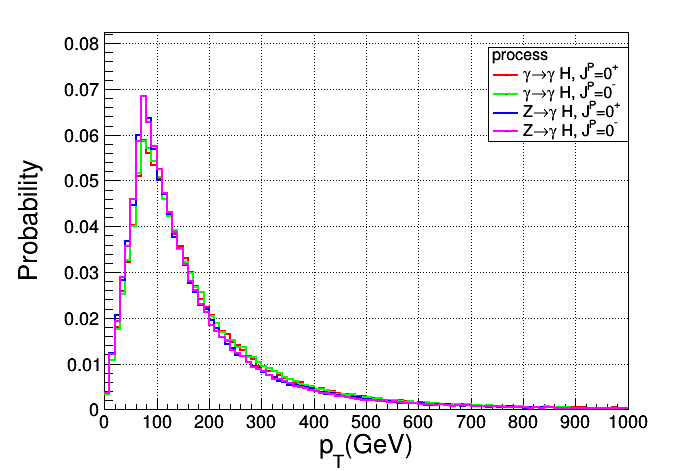
\includegraphics[width=0.45\textwidth]{./figures/h_pt}}
\end{figure}
\end{frame}


\begin{frame}
\frametitle{Kinematics of photon}
\begin{figure}[H]
\setcounter{subfigure}{0}
\centering
\subfloat[Distribution of photon $\eta$ ]{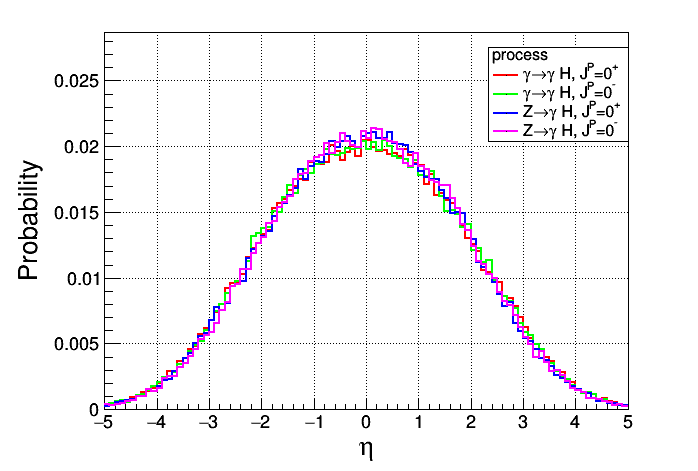
\includegraphics[width=0.45\textwidth]{./figures/ph_eta}} 
\subfloat[Distribution of photon $p_T$ ]{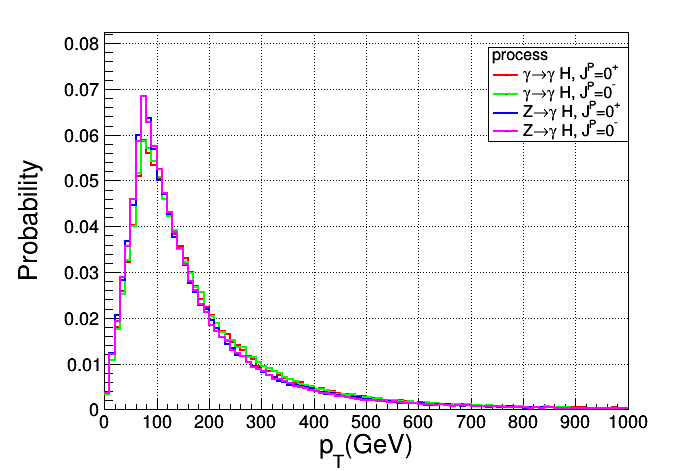
\includegraphics[width=0.45\textwidth]{./figures/ph_pt}}
\end{figure}
\end{frame}

\begin{frame}
\frametitle{Kinematics}
\begin{figure}[H]
\setcounter{subfigure}{0}
\centering
\subfloat[Distribution of $\Delta\eta_{\gamma H}$ ]{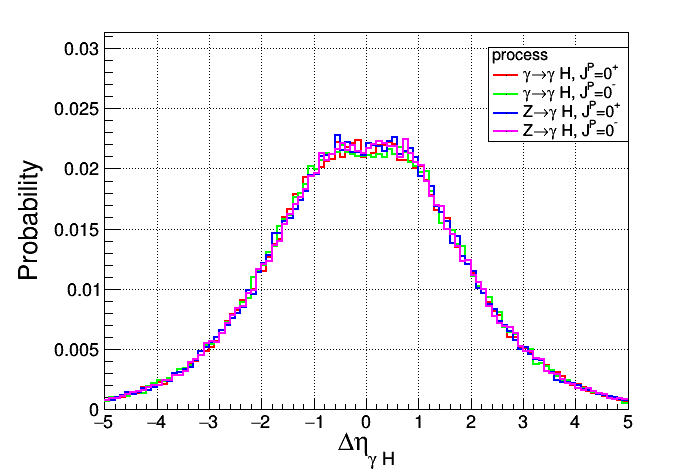
\includegraphics[width=0.45\textwidth]{./figures/delta_eta}} 
\subfloat[Distribution of invariant mass ]{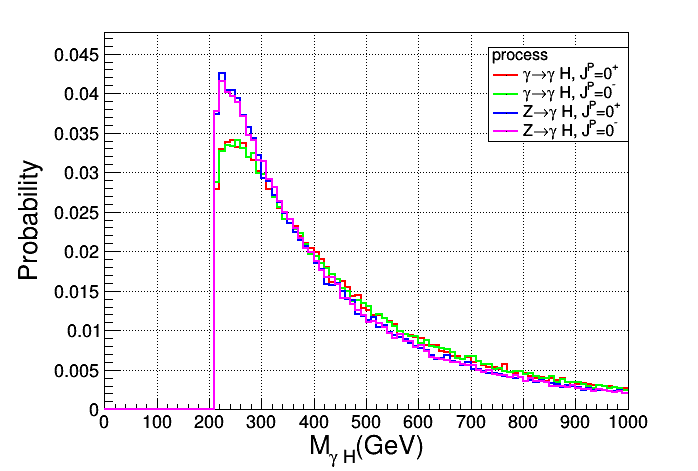
\includegraphics[width=0.45\textwidth]{./figures/M_gammah}}
\end{figure}
\end{frame}

%------------------------------------------------
\iffalse
\begin{frame}
\Huge{\centerline{The End}}
\end{frame}
\fi
%----------------------------------------------------------------------------------------

\end{document} 